\section{设计思路}

\subsection{DeepFM}

本算法主要基于Guo等人的DeepFM模型\cite{guoDeepFMFactorizationMachineBased2017}进行改进。
自DeepFM模型提出以来,
迅速在推荐系统领域成为最受欢迎的算法之一,
其主要基于Google的Wide \& Deep模型,
将Wide部分使用FM进行特征提取,
获得了不错的性能同时也有较高的准确率。
其算法的主要结构如\cref{fig:deepfm}所示。

\begin{figure}[!htbp]
	\centering
	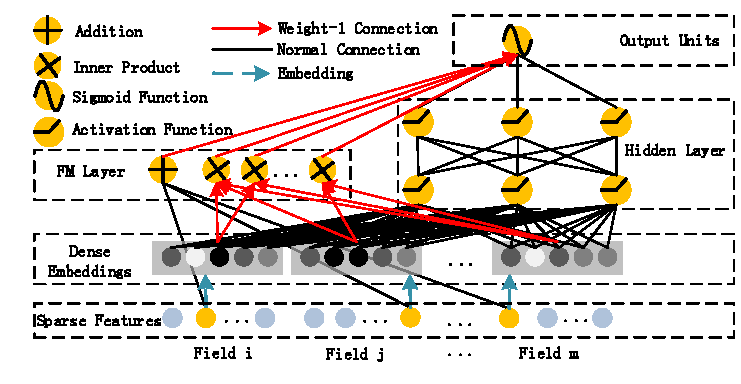
\includegraphics[width=.9\textwidth]{images/architecture-deepfm.pdf}
	\caption{DeepFM}\label{fig:deepfm}
\end{figure}

其主要用于对离散型变量进行训练。
将OneHot编码使用嵌入层嵌入后分别用FM和DNN进行训练,
最终FM和DNN的结果相加后输出。

但是在游戏推荐领域,
往往有非常多的标签数据、
连续型数据例如游玩时间等。
如果使用DeepFM模型,
往往会造成模型过于庞大的问题,
对于大量用户产生的数据,
往往会由于模型复杂度提升而耗费大量的计算资源,
对于对服务器有一定要求的游戏领域往往需要
额外的大量计算资源进行模型的训练。
上述问题均是DeepFM所无法解决的,
因此需要一种新的算法来进行优化,
以尽可能减少计算资源。

\subsection{算法改进}

考虑到DeepFM对标签类型数据需要当作大量OneHot编码,
使得数据过于稀疏,
同时模型的复杂度过高,
不便于进行计算。
因此,
对于标签数据的嵌入层部分选择使用Word2Vec进行词嵌入。
词嵌入部分可以作为预训练部分进行处理,
同时其训练速度非常快,
对计算资源的占用不高。
对于稀疏数据,
选择将与DeepFM类似的方法,
将嵌入层数据交由FM与线性层分别处理,
并将其与嵌入层数据一并输出,
最终将Word2Vec、连续数据与词嵌入数据一并使用
神经网络进行训练,
最终进行输出。
算法的大概框架如\cref{fig:model}所示。

\begin{figure}[!htbp]
	\centering
	\includegraphics[width=.9\textwidth]{images/model.pdf}
	\caption{模型设计}\label{fig:model}
\end{figure}

算法的具体设计可见\cref{sec:design}.